%sse
\documentclass[../../main/main.tex]{subfiles}


\begin{document}
\title{Systems Security Engineering}


%%%%%%%%%%%%%%%%%%%%% Chapter CSBD ACL %%%%%%%%%%%%%%%
\chapter{Systems Security Engineering \& Patrol Base Operations}\label{chp:sse}


       %%%%%%%%%%%%%%%%%% Section Systems %%%%%%%%%%%%%%%%
\section{The Systems Perspective}\label{sec:systems}
A system is a set of interacting and interdependent components that act as a whole to perform some behavior or function.  Examples of systems include the human body, socio-political systems, and computer systems. 

The patrol base operations satisfy this definition of a system.  As a whole, the patrol base operations perform some function(s).  This function is described in the Ranger Handbook \cite{rangermanual} and discussed in chapter \ref{chp:pb}.  The patrol base operations are comprised of interdependent and interacting components.  In general these components are the individual soldiers.  But, the way this master thesis defines the patrol base operations, the definition of a component varies.

This master thesis defines the patrol base operations as a system of systems.  More specifically, this thesis models the patrol base operations as a hierarchy of \glsentrylongpl{ssm}.  Chapter \ref{chp:ssmmodel} describes \glsentryshortpl{ssm} in general.   Section \ref{sec:modelingpb} describes this model of the patrol base operations.  

This model presents the patrol base operations as a hierarchy wherein each level of the hierarchy represents a decreasing level of abstraction.  At the top and most abstract level, the components are phases of the patrol base operations.  These phases commence in a sequential order to achieve the goal of the patrol base operations.  Each lower level of the hierarchy is composed of less abstract phases. At each level, the components function sequentially (typically) to achieve the ultimate goal.  

This system of systems also contains non-hierarchically defined components.  For example, an escape-level component models situations wherein the patrol base operations are aborted.  The escape level component is reachable from any component at any level of the hierarchy.  Soldiers (as in a soldier model) also function within this system of systems in a non-hierarchical manner.  However, the soldier module is not verified using the \glsentryshort{acl} because of time constraints.   Nevertheless, a soldier module is discussed in the Discussions chapter \ref{chp:discussion} of this thesis.

In this way, the patrol base operations represent a system and are amiable to the systems engineering perspective.  

     %%%%%%%%%%%%%%%%%% Section Systems Engineering %%%%%%%%%%
\section{Systems Engineering}\label{sec:se}
The recognized authoritative standard on systems engineering is ISO/IEC/IEEE 15288 \cite{iso15288}.  This document is titled "Systems And Software Engineering--System Life Cycle Processing."  A precursor to this standard is ISO/IEC TR 24748 1 \cite{iso24748} titled "Systems And Software Engineering--Life Cycle Management--Part 1: Guide for Life Cycle Management."   These are the primary sources for this section.

Systems engineering is an interdisciplinary approach aimed at solving problems involved in the various phases of the life cycle of a system.  ISO/IEC/IEEE 15288 and ISO/IEC TR 24748 1 define five major phases of the this life cycle: concept, development, production, utilization, support, and retirement.
  
This master thesis focuses on the \glsentrylong{csbd} (\glsentryshort{csbd}).  The key premise of \glsentryshort{csbd} is that security should be built into the systems from the start, i.e., the design phase.  This is the leading notion in systems engineering and its sub-discipline \glsentrylong {sse}.  Nevertheless, it is instructive to see how CSBD, this thesis, and the patrol base operations fit into the systems engineering framework described by the ISO standards.

\paragraph*{Concept} 
The concept phase describes stakeholders and the \glsentrylong{conops} (ConOps).  Stakeholders are those who have a stake in the system.  ConOps are defined in a variety of ways.  Wikipedia defines ConOps as "...a document describing the characteristics of a proposed system from the viewpoint of an individual who will use that system \cite{wikiconops}.  U.S. Air Force Policy Directive 10-28 defines ConOps as "a high level concept whose purpose is to describe operational mission areas, enablers and effects necessary to achieve desired results/outcomes" \cite{af1028}.  ConOps are context specific.  

The patrol base operations are already modeled and implemented. The mission areas, enablers, and effects to achieve the desired goal are already in place.  The aim for this thesis is to maintain the structure of the patrol base operations and model it in a way that is amiable to verification and documentation of complete mediation.

It is possible to look at the work in this thesis as the modification of an already in-use system. For example, an accountability system involving the patrol base operations may require a remodeling of the operations with few, if any, changes in the actual operations themselves.  This is discussed in more detail in the Future Works \& Implications Chapter in section \ref{sec:accountability}.

\glsentrylong{csbd} (CSBD) applies to these two areas: the concept phase and the re-conceptulaization phase.
 
\paragraph*{Development}
The development stage involves refinement of the ConOps and production of products.  The development of the patrol base operations took place a long time ago.  Regardless, the products for the patrol base operations are the description of the operations themselves. The product with regards to this master thesis is demonstrated satisfaction of the principle of complete mediation.

\glsentryshort{csbd} does not add anything new to the development of the system.  However, it adds constraints to the concept phase which must be adhered to throughout the development phase.

\paragraph*{Production}
Production is self-explanatory, however not so obvious with a system such as the patrol base operations.  There are no products save for the trained soldier.  In this aspect, the production phase would entail educating the soldiers.  Neither this master thesis nor \glsentryshort{csbd} cover\footnote{Although, CSBD is a required course at Syracuse University in the Cyber Security program.} education of soldiers. (Of course, one could imagine a lecture on the importance of authentication and authorization as a critical component of any soldier's primary training.)

\paragraph*{Utilization}
Utilization is also self-explanatory.  The patrol base operations are utilized in the field as soldiers are deployed and assigned missions that involve patrol base operations. Again, neither this master thesis nor \glsentryshort{csbd} focus on utilization.

\paragraph*{Support}
Support provides for maintenance of the system.  In the case of the patrol base operations, support would entail documenting feedback from soldiers and assessing the efficacy of the operations.  This could also entail updating the operations based on this feedback and based on advances in technology.  Neither this master thesis nor \glsentryshort{csbd} directly address support for the system.  However, any updates to the system would likely entail consideration of authentication and authorization. Herein, this master thesis and \glsentryshort{csbd} are relevant and useful.

\paragraph*{Retirement}
Retirement refers to the end stages of the operations.  For the patrol base operations and similar systems, retirement would most likely entail replacement with other operations.  Again, neither this master thesis nor \glsentryshort{csbd} focus on retirement.  However, both are be relevant to the conceptualization of the replacement system.

     %%%%%%%%%%%%%%%%%% NIST %%%%%%%%%%%%%%%%%%%%%
\section{NIST Special Publication 800-160}
One work in the field of \glsentrylong{sse} is such a critical component to the field of \glsentryshort{sse} that it warrants pointing out. The \glsentrylong{nist} (NIST) defines its mission as such: "To promote U.S. innovation and industrial competitiveness by advancing measurement science, standards, and technology in ways that enhance economic security and improve our quality of life." \cite{nistmission}.  As their name suggests, NIST develops standards for various industries of relevance to the nation.   

The relevant standard for \glsentrylong{sse} (\glsentryshort{sse}) is NIST Special Publication 800-160 Volumes 1 and 2. The title of volume 1 is "Systems Security Engineering
Considerations for a Multidisciplinary Approach in the Engineering of Trustworthy Secure Systems."  The title of volume 2 is "Systems Security Engineering Cyber Resiliency Considerations for the Engineering of Trustworthy Secure Systems."   These, in particular volume 1, are the primary sources for the following two sections.  

     %%%%%%%%%%%%%%%%%% Section Systems Security Engineering %%%%%%
\section{Systems Security Engineering}\label{sec:sse} 
Systems security engineering (\glsentryshort{sse}) is a sub-discipline of systems engineering.  Figure \ref{fig:nist800160} shows \glsentryshort{sse} in relation to systems engineering and other sub-disciplines of \glsentryshort{sse}.  This master thesis falls into one of the Security Specialties in this diagram.

\begin{figure}[h]
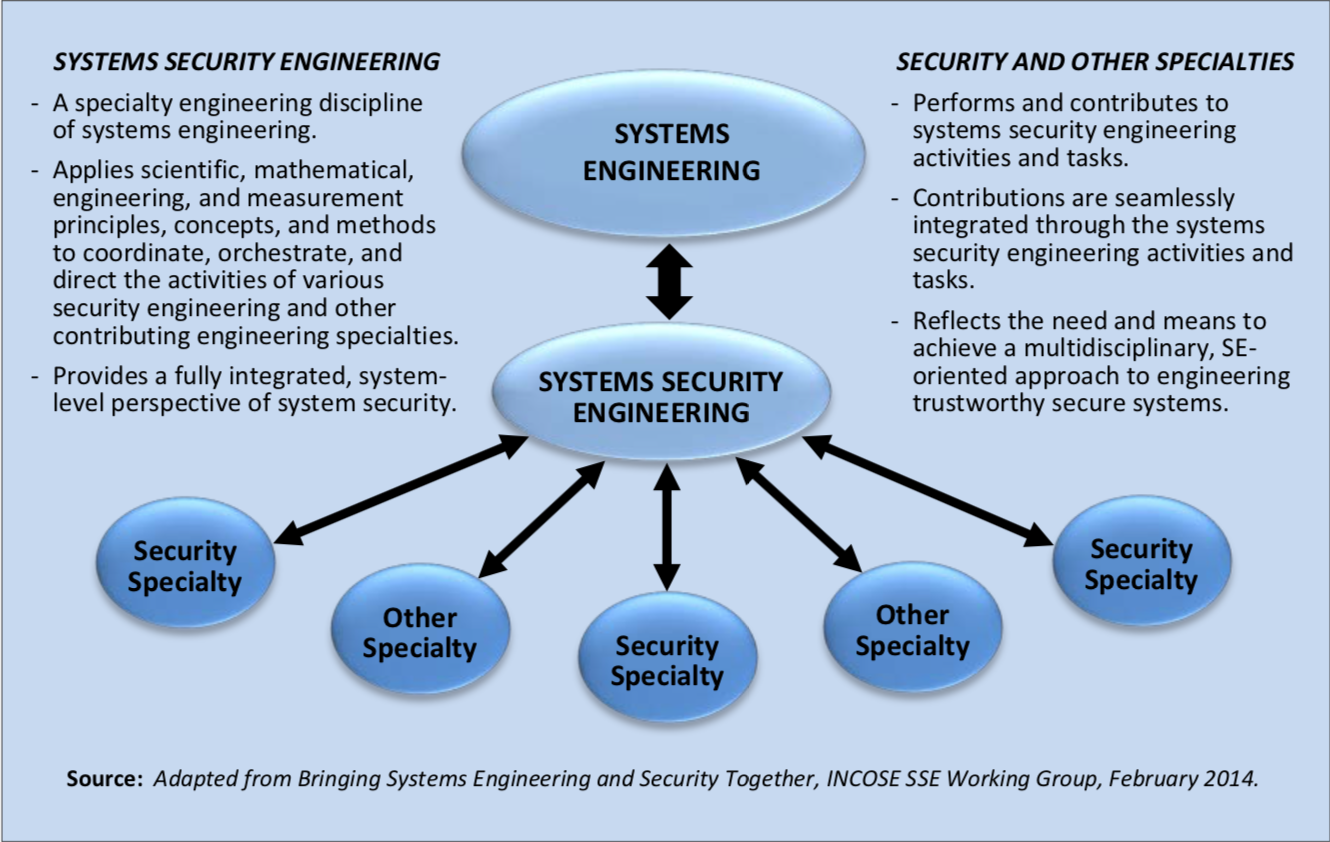
\includegraphics[width=\linewidth]{../figures/seincontext.png}
\caption{\label{fig:nist800160}Systems security engineering in relation to systems engineering. (Image from \glsentryshort{nist} Special Publication 800-160: Systems Security Engineering Considerations for a Multidisciplinary Approach in the Engineering of Trustworthy Secure Systems.)}
\end{figure}

According to \glsentryshort{nist} Special Publication 800-160, "Systems security engineering focuses on the protection of stakeholder and system assets so as to exercise control over asset loss and the associated consequences."  Three key concepts in \glsentryshort{sse} are stakeholder, asset, and unacceptable losses.  In modeling the patrol base operations, this thesis first defines these key concepts.  

\begin{description}
\item[ Stakeholder]  The stakeholder governs the ConOps and conceptualization of the system.  The stakeholder defines what the system should do.  The stakeholder also defines what the system should not do and what are unacceptable losses.  The stakeholder for the patrol base operations are ultimately the U.S. military.  But, this thesis has a different purpose, that of demonstrating specific security properties of the patrol base operations using CSBD.  For this master thesis, the stakeholders can be thought of as those who are funding and managing this research (see the Acknowledgements section).  The ConOps for this model of the patrol base operations require that the system should be modeled in a way amiable to verification of complete mediation.


\item[Asset] An asset is anything that is of value to the stakeholder.   In the patrol base operations, this includes soldiers, equipment, and the mission.  For this master thesis, the assets remain the same.  But, they also include phases (or states) of the model.  These can be thought of as sub-missions.

\item[Unacceptable losses] Unacceptable losses are self-defining.  Unacceptable losses for the patrol base operations are defined broadly as any event that would cause the patrol base operation as a whole to abort.  These are: contact with the enemy, casualties, a change in mission from higher-up.  Unacceptable losses from the perspective of this master thesis include situations wherein complete mediation can not be verified.  In these cases, the model should be revised until it does satisfy the property of complete mediation.
\end{description}

It is a critical objective of \glsentryshort{sse} to identify assets and unacceptable losses according to the stakeholder, and then design the system in a way that minimizes asset loss and avoids unacceptable losses.  This thesis begins with an assumption that these are already explored in the original design of the patrol base operations (see Ranger Handbook \cite{rangermanual}).  This also means that this thesis assumes that the security properties of the patrol base operations are already built-in to the design.  These assumptions are necessary because the goal of this thesis is not to design the patrol base operations, but to describe them in manner amiable to verification of complete mediation.  Ideally, this would be applied to any future such operations during their inception.  

Nevertheless, this master thesis includes the unacceptable losses described above in this model...because they are part of the patrol base operations.  To cover the unacceptable losses, this master thesis models an escape-level \glsentrylong{ssm} (SSM).  If at any phase in the patrol base operations any authenticated principal (i.e., the platoon leader) reports an abortable event, the escape-level \glsentryshort{ssm} will abort the patrol base operations. This includes casualties or unacceptable equipment failure.  By creating one escape-level \glsentryshort{ssm}, this thesis creates a modularized yet expandable treatement of unacceptable losses.


To further describe the model of the patrol base operations in the context of \glsentryshort{sse}, a few more concepts are necessary.  

\section{Systems Security Engineering Framework}\label{sssec:sseframework}
NIST 800-160 describes the systems security engineering framework shown in figure \ref{sseframework} as "contexts within which systems security engineering activities are conducted."  CSBD focuses primarily on demonstrating trustworthiness.  Nevertheless, this master thesis also addressed other aspects of the framework.  

\begin{figure}[h]
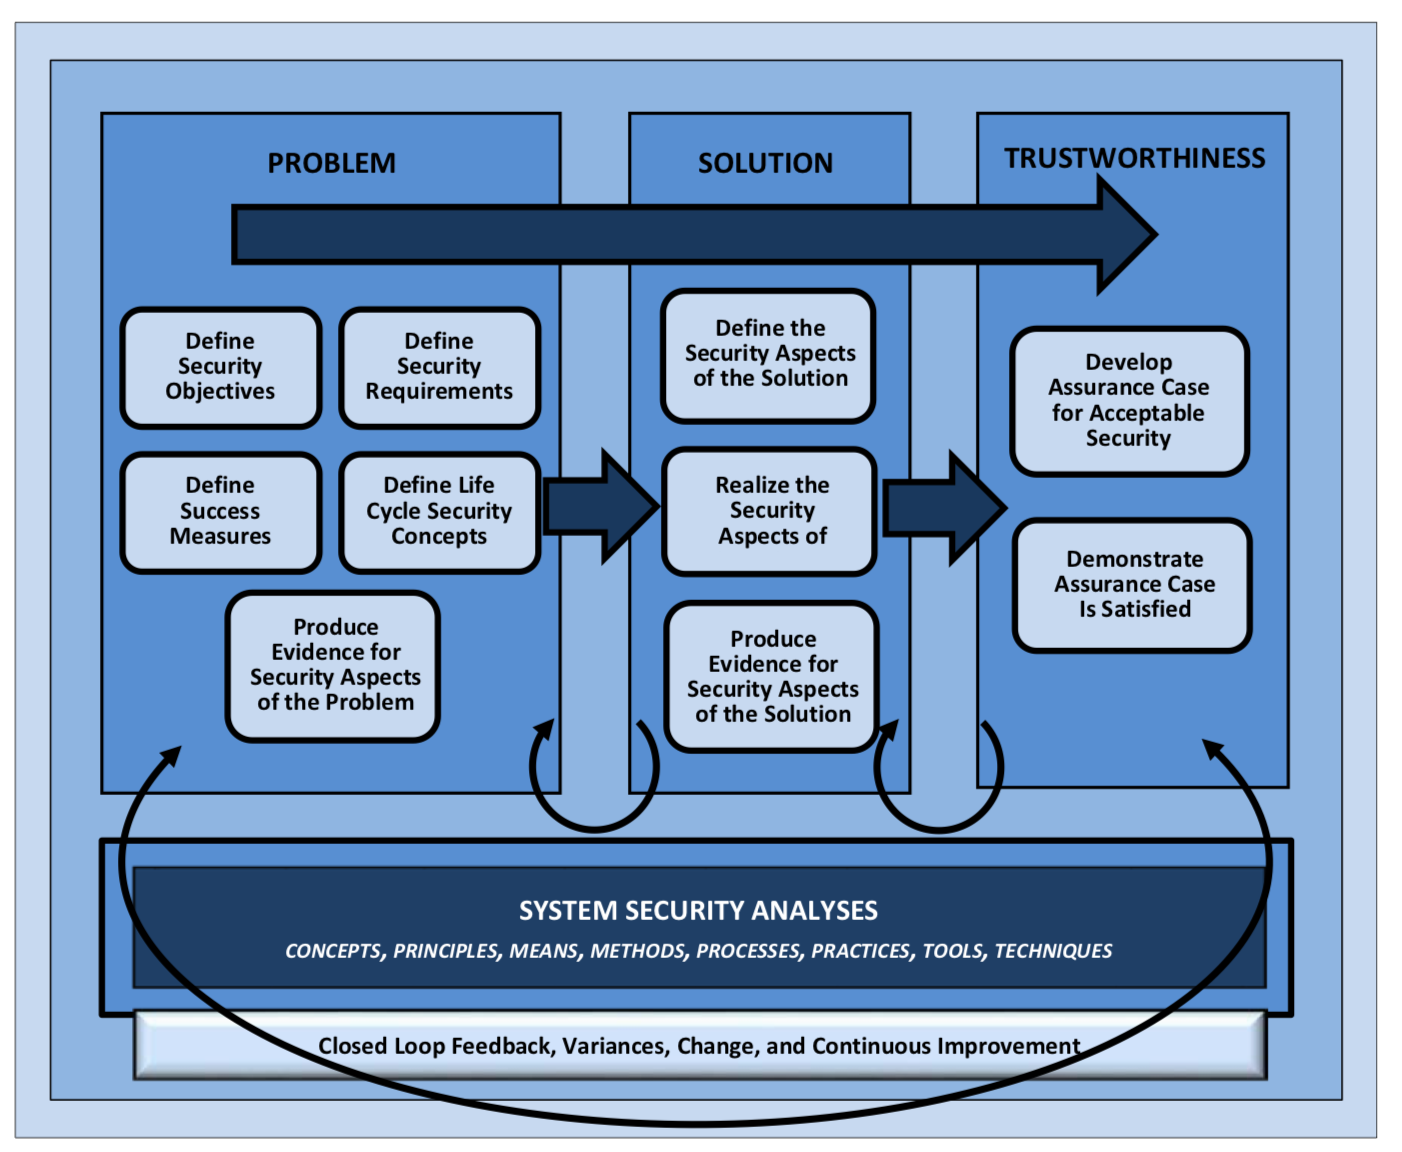
\includegraphics[width=\linewidth]{../figures/sseframework}
\caption{\label{sseframework}Systems security engineering Framework. (Image from \glsentryshort{nist} Special Publication 800-160: Systems Security Engineering Considerations for a Multidisciplinary Approach in the Engineering of Trustworthy Secure Systems.)}
\end{figure}

The problem and solution phases for the patrol base operations take a different approach in the context of this master thesis. It is not our goal to outline the potential security threats and then to find solutions for them.  This was, hopefully, already done when the patrol base operations were originally defined.  Nonetheless, it is necessary to identify the problem and solution within the patrol base operations in order to verify their security properties.  


\subsection{Problem}
A problem (or goal) for any Ranger operation is suggested by the following statement in the Ranger Handbook  \cite{rangermanual}: "To survive on the battlefield, stealth, dispersion, and security is enforced in all tactical movements." Thus, enforcing security is a primary problem inherent in the patrol base operations.  This is very relevant to the goal of this master thesis and more generraly \glsentryshort{csbd} approach.  

\glsentryshort{csbd} focuses on a subspecialty in \glsentryshort{sse}, that of complete mediation.  In the conceptualization of any real system, \glsentryshort{csbd} would be applied in conjunction with other subspecialty areas of \glsentryshort{sse}.  But, for this thesis, the problem at hand is to model the patrol base operations in a way that is amiable to verification of complete mediation.

The problem inherent to the application of complete mediation is defining the objects to be accessed.  Complete mediation refers to control over who or what has access to these objects.  Thus, the protected objects must be clearly defined.

We the problem defined, this master thesis moves on to the solution phase.



\subsection{Solution}
The simplest solution to this problem is to model the patrol base operations as a hierarchy of secure state machines (\glsentryshort{ssm}).  The hierarchy simplifies the design of the solution by creating decreasing levels of abstraction with multiple modules at each level.  This allows for focus on one level and one module at time. This essentially amounts to a system of systems approach.  Furthermore, this allows for greater separation of work.  After one level of the hierarchy is complete, CSBD is applied to that level while the next level of the hierarchy is being designed.

\glsentryshortpl{ssm} are readily defined with complete mediation embedded into their design.  \glsentryshortpl{ssm} are discussed in detail in Chapter \ref{chp:ssmmodel}\footnote{In fact, a parametrizable model of an \glsentryshort{ssm}\footnote{This SSM was modeled and implemented in HOL by Professor Shiu-kai Chin and used with his permission.} was already designed and implemented in \glsentryshort{hol} prior to the start of this project.  The constraints of this project suggested Improvements\footnote{Because these improvements were significant, the original author (Professor Shiu-kai Chin) made them.} to this parametrizable \glsentryshort{ssm}Much to the chagrin of the author, a significant portion of the SSMs had to be redone with the new parametrizable SSM.}.

The objects to be accessed varies at each level of abstraction. At the top and most abstract level, the objects are the transitions.  That is, control over the transitions between phases (or states) of the patrol base operations are to be protected.  Objects are defined similarly for each module and at each level for the entire hierarchy of the model.  These are deducible from the descriptions of each module (or \glsentryshort{ssm}) in their appropriate section (see section \ref{ssec:omnilevel} to start).  For the sake of brevity, this section only discusses the top level to illustrate the key concepts.  

The accessors are the leaders designated at each level of abstraction.  The best way to negotiate access to objects is by the principle of least privilege.  This principle assigns privilege to only those who are deemed necessary and to no others.  At the top level, the platoon leader (and only the platoon leader) is designated as the accessor. This means that only the platoon leader can issue commands to move-on to the next phase (or state) in the patrol base operations. Some of the other modules have more than one accessor.  These accessors are typically assigned privileges to specific objects within the module.  The rights of each accessor are determined by the policy.

In the real patrol base operations, soldiers recognize each other by face.  Thus, it is sufficient to just authenticate the platoon leader at each level without requiring any passwords or other means of authentication\footnote{The author and subject matter expert discussed authentication in the context of an accountability system wherein passwords or chips were required for authentication.  But, we did not implement such authentication techniques in this project.}.

Policy is determined for each module and at each level of the patrol base operations model.  The model includes not only "who" is authorized to do what, but also what preconditions are necessary prior to authorization.  This is more complicated than authentication.

At the top level, there are only two requirements for the patrol base operations to move to the next phase of the operations: (1) the previous phase is complete, and (2) the platoon leader issues the command to move to the next phase.  This creates a potential conflict between the goal of modularizing each component and creating a hierarchy wherein each level of the hierarchy expands upon the one above it.  In general, If the top level requires some signal from the lower level that it is complete, then these two levels are not independent. 

To solve this problem, an OMNI level module is created.  The OMNI level module is thought of as all-knowing.  This module relays information from all modules as needed.  With this construct, the top level does not need to "know" if the lower level module is complete.  It only needs to know that the OMNI level says that it is complete.  The OMNI level is given the authority to determine when any module is complete.


With this solution in mind, the top level policy looks like this.
\fbox{
\parbox{\linewidth}{
\begin{center}
\textit{if OMNI-Level says the previous phase is complete\footnote{For those who have read ahead, the reader may recognize that this does not follow logically from the inference rules.  The actual implementation of this policy requires the two inputs on the first and second line and returns that output on the final line.  Within the policy is the requirement that OMNI Level has the authority to determine that the previous phase is complete.  To state this in the text here would only clutter it and confuse the reader.}, and \\
Platoon Leader says move to the next phase\\
 then Platoon Leader has the authority to move to the next phase}
\end{center}
}}

The most useful property of the \glsentryshort{ssm} is that complete mediation is made a condition for transitions among states.  That is, to transition from one state to another the accessor (requestor) must be properly authenticated and authorized.  For example, at the top level, transition commands in an \glsentryshort{ssm} look like this.

\fbox{
\parbox{\linewidth}{
\begin{center}
\textit{if Platoon Leader's identity is authenticated, and\\
         Platoon Leader says move to the next phase, and \\
         Platoon Leader has the authority to move to the next phase\\
         then move to the next phase.}
\end{center}
}}

The first line ensures authentication of the Platoon Leader.  The second line is a request from the Platoon Leader to access the object (i.e., move to the next phase).  The third line is the output of a policy shown in the box above. The final line is the conclusion which justifies transition to the next phase.

Note that this is an "if and only if" conditional.  This means that if the Platoon Leader is authenticated, authorized on, and issues the command then the command is executed.  It also means the converse.  If the command is executed, then the Platoon Leader is authenticated, authorized on, and issues the command to do so.  The former is required for transitions to occur.  The later (converse) is critical for accountability.  

\subsection{Trustworthiness}
NIST SP 800-160 states that \textit{assurance cases} are the basis for trustworthy context.  It states, "An assurance case is a well-defined and structured set of arguments and a body of evidence showing that a system satisfies specific claims with respect to a given quality attribute." The key points here are that the assurance case must be clearly defined and also clearly demonstrated. 

Trustworthiness in the context of this master thesis and more generally \glsentryshort{csbd} means that all protected objects are accessed if and only if that accessor is both authenticated and authorized.  The processes of authentication and authorization are clearly defined in the Solution section above.  Therefore, what remains is to demonstrate that actually does what it claims to do.  This is where the \glsentrylong{acl} (ACL) and computer-aided reason take center stage.  

A key concern in \glsentrylong{sse} (SSE) is measuring trustworthiness.  For this thesis and \glsentryshort{csbd}, trustworthiness is measured by whether or not the system satisfies the principle of complete mediation. The evidence that it does is formally verified proofs using an access-control logic (\glsentryshort{acl}).  The \glsentryshort{acl} is described in detail in chapter \ref{chp:csbdacl}.  Application of \glsentryshort{acl} to the patrol base operations follows that chapter.    

In essence, the \glsentryshort{acl} formally describes the informal logic shown in the two boxes in the Solution section.  This logic is implemented in the \glsentrylong{hol} (HOL) Interactive Theorem Prover.  In addition, the hierarchy of state machines are described in \glsentryshort{hol}.  With these, it is possible to prove theories in \glsentryshort{hol} that pertain to complete mediation.  These are formal proofs generated by a trusted theorem proving assistant.  

With these proofs, it is accepted that the model of the patrol base operations satisfies the principle of complete mediation.  These are considered demonstrated proofs, or assurance cases, 

\section{Verification \& Documentation}\label{sssec:sseframework}
\subsection{Verification}
Verification amounts to proof of trustworthiness.  NIST SP 800-160 often refers to "security-focused" verification.  Verification is built-in to the \glsentryshort{csbd} method.  It focuses on the use of authentication and authorization in the design of the system.  \glsentryshort{csbd} demonstrates is usefulness not only a guide to complete mediation, but also as a tool that applies formal methods using computer-aided reasoning to verify any claims of complete mediation. This is referred to as formal verification. Thus, \glsentryshort{csbd} is a complete approach to designing trustworthy systems.

\subsection{Documentation}
A common concept in science and engineering is "if you didn't document it then it didn't happen."  Documentation is specifically important to claims of trustworthiness because such claims are not always readily apparent in the system. Systems may run smoothly without adequate security ... until something finally goes wrong?  Then, everyone scrambles to find the cause of the problem.

Documentation is often the least exciting aspect of systems engineering. But, documentation is one of the most important activities in the systems engineering processes.  Most people find that documentation reveals aspects of the system that are overlooked.  It checks the accuracy of the work.  Documentation describes the system for posterity and communicates the system for the benefit of others.  

\subsubsection{Accountability}\label{ssec:accountability}
Internet Hall of Fame Inductee Vint Cerf commented on the importance of accountability in \glsentryshort{sse} at a recorded conference in 2016.  The conference titled "Exploring the Dimensions of Trustworthiness: Challenges and Opportunities" is presented by NIST.  Accountability is incredibly important.  When things go wrong, the first thing that people do is ask "what happened and who is responsible."


Documentation is a great accountability tool.  Documentation demonstrates that the system is realized to the satisfaction of the stakeholders. If something goes wrong, documentation aids in tracing the source of the problem. It saves time and resources to identify and eliminate areas where security is adequately demonstrated.   Furthermore, everyone wants to document their work for their in protection, in case something does go wrong.  

Documentation is a primary component of \glsentryshort{csbd}.  The \glsentryshort{hol} formal proofs are all printable. It is standard to generate a printout of all theories and generate a pdf.  

\subsubsection{Reproducibility}\label{ssec:reproducibility}
In addition to formal verification and documentation of complete mediation, all proofs are fully reproducible.  The \glsentrylong{acl} proofs can be worked-out by hand.  In addition to \glsentryshort{hol}, \glsentryshort{acl} can also be implemented in other theorem provers.

\end{document}